\begin{abcliste}
\abc Die Skizze ist massstäblich. Die Erde steht im Brennpunkt der Übergangsellipse; Perigäum und Apogäum liegen sich gegenüber.

\begin{center}
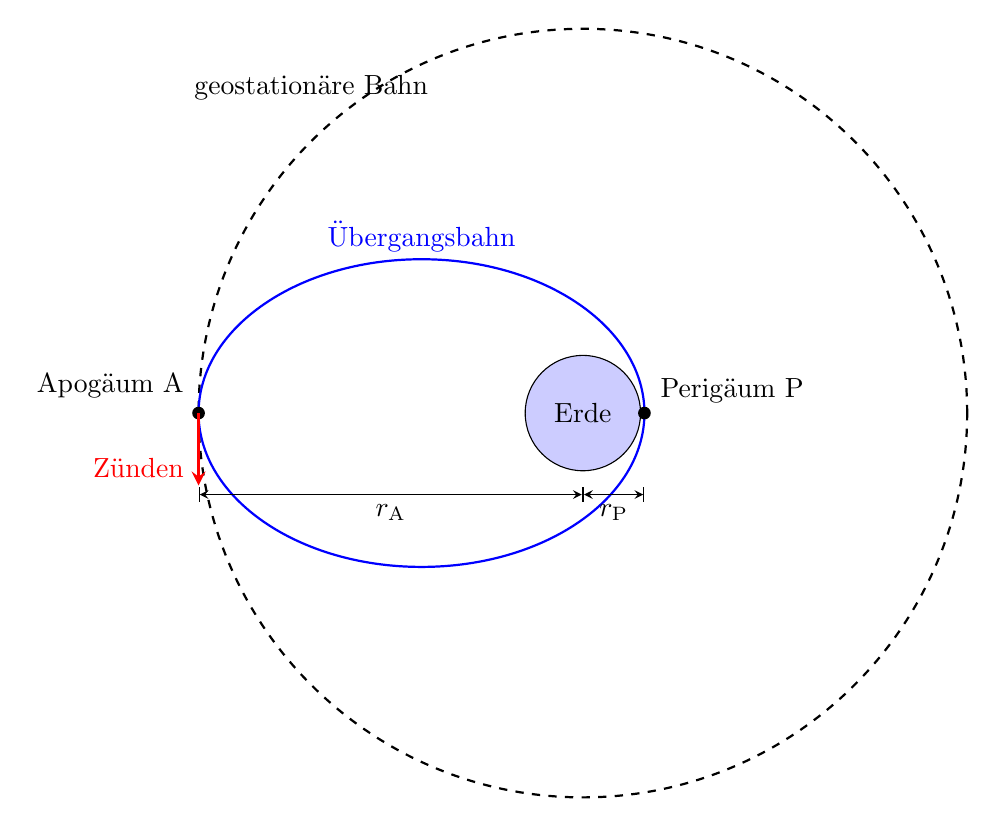
\begin{tikzpicture}[>=stealth, scale=1.15]
 \draw[dashed, thick] (0,0) circle (4.244);
 \node at (-3.0,3.6) {geostationäre Bahn};
 \draw[blue, thick] (-1.782,0) ellipse (2.462 and 1.699);
 \node[blue] at (-1.782,1.95) {Übergangsbahn};
 \fill[blue!20] (0,0) circle (0.637);
 \draw (0,0) circle (0.637);
 \node at (0,0) {Erde};
 \fill (0.68,0) circle (0.07);
 \node[anchor=west] at (0.75,0.25) {Perigäum P};
 \fill (-4.244,0) circle (0.07);
 \node[anchor=east] at (-4.3,0.3) {Apogäum A};
 \draw[|<->|] (0,-0.9) -- (0.68,-0.9) node[midway, below] {$r_\mathrm{P}$};
 \draw[|<->|] (-4.244,-0.9) -- (0,-0.9) node[midway, below] {$r_\mathrm{A}$};
 \draw[->, very thick, red] (-4.244,0) -- (-4.244,-0.8);
 \node[red, anchor=east] at (-4.3,-0.6) {Zünden};
\end{tikzpicture}
\end{center}

\abc Perigäum und Apogäum liegen sich auf der grossen Achse gegenüber, also
\begin{align}
 a &= \aHF = \frac{\rpH+\rAH}{2} = \aH \approx \result{\aHP{3}{3}}
\end{align}
Im Apogäum ist die Gesamtenergie die Summe aus kinetischer Energie und Gravitationsenergie:
\begin{align}
 \frac{1}{2}\,m_\mathrm{S}\,v_\mathrm{A}^2-G\,\frac{M_\mathrm{E}\,m_\mathrm{S}}{r_\mathrm{A}} &= -\frac{1}{2}\,\frac{G\,M_\mathrm{E}\,m_\mathrm{S}}{a}
\end{align}
Mit $M_\mathrm{E} = \MErO$ (FoTaBe S.~209) folgt
\begin{align}
 v_\mathrm{A} &= \vAHF \\
   &= \sqrt{\ncG\cdot\MEr\cdot\left(\frac{2}{\rAH}-\frac{1}{\aH}\right)} \\
   &= \vAH \approx \result{\vAHP{3}{3}}
\end{align}

\abc Auf der geostationären Kreisbahn mit Radius $r_\mathrm{A}$ ist die Gravitationskraft die Zentripetalkraft, $G\,M_\mathrm{E}\,m_\mathrm{S}/r_\mathrm{A}^2 = m_\mathrm{S}\,v_\mathrm{K}^2/r_\mathrm{A}$:
\begin{align}
 v_\mathrm{K} &= \vKrF = \sqrt{\frac{\ncG\cdot\MEr}{\rAH}} = \vKr
\end{align}
Die Raketen müssen die Geschwindigkeit also erhöhen um
\begin{align}
 \Delta v &= \dvHF = \vKr-\vAH = \dvH \approx \result{\dvHP{3}{2}}
\end{align}
\end{abcliste}
